	\documentclass[
		a4paper,	% Dimensão do documento
		12pt,		% Tamanho default de fonte
		]{article}	% Classe do documento

	% CODIFICAÇÕES E FONTES
	\usepackage[utf8]{inputenc} % Codificação de caracteres
	\usepackage[T1]{fontenc}    % Codificação de fontes
	\usepackage{kpfonts}	    % Fonte Kepler
	\usepackage[brazil]{babel}  % Português brasileiro como idioma padrão

	% FORMATAÇÃO
	\usepackage{geometry}	% Modificar margens
		\geometry{
			left=20mm,		% Margem esquerda
			right=20mm,		% Margem direita
			top=25mm,		% Margem superior
			bottom=25mm,	% Margem inferior
			}
	\usepackage{microtype}	% Melhora tipografia
	\usepackage{setspace}	% Permite definir espaçamento entre linhas
		\renewcommand{\baselinestretch}{2.0}	% Espaçamento duplo como default

	% GRÁFICOS E FIGURAS
	\usepackage{graphicx}	% Para inserir imagens
	\graphicspath{
		{/home/gustavo/Documentos/Universidade/Unicamp/master-research/images/} }
	\usepackage{tikz}		% Para criar ilustrações
\usepackage[labelfont={sc}]{caption}
	% CORES
	\usepackage{xcolor}	% Permite usar cores
		\definecolor{azul}{HTML}{0b365a}		% Azul
		\definecolor{verde}{HTML}{004d00}		% Verde
		\definecolor{vermelho}{HTML}{B20000}	% Vermelho
		\definecolor{cinza1}{HTML}{DCDCDC}		% Cinza 1
		\definecolor{cinza2}{HTML}{A9A9A9}		% Cinza 2

	% HYPERREF
	\usepackage[
		colorlinks=true,	% Texto colorido ao invés de frame
		linkcolor=vermelho,	% Cor de referências internas
		citecolor=azul,		% Cor de citações
		filecolor=magenta,	% Definir cor de links que abrem arquivos locais (?)
		urlcolor=verde,		% Cor de links externos (urls, emails)
		pdftitle={			% Título que aparece na janela do visualizador
			Acomodação dialetal na dimensão rítmica da fala
			},
		bookmarks=true,		% Mostrar bookmarks ao abrir o documento
		]{hyperref} 

	% TABELAS E LISTAS
	\usepackage{array}		% Mais recursos nos ambientes array e tabular
	\usepackage{booktabs}	% Mais recursos para criação de tabelas
	\usepackage{multicol}	% Permite aglutinar cédulas na dimensão da coluna
	\usepackage{multirow}	% Permite aglutinar cédulas na dimensão da linha
	\usepackage{colortbl}	% Colorir tabelas
	\usepackage{dcolumn}	% Esqueci a função deste pacote
	\renewcommand{\arraystretch}{1.3} % Espaçamento de linhas em tabelas
	\usepackage[
		ampersand,	% Define como caractere '&' como operador
		]{easylist}	% Facilita a criação de listas mais complexas

	% MATEMÁTICA
	\usepackage{amsmath}	% Pacote para expressões matemáticas

	% BIBLIOGRAFIA E CITAÇÃO
	\usepackage[ 
			backend=biber,			% Compilador de bibliografia
			style=authoryear,		% Estilo de bibliografia
			citestyle=authoryear,	% Estilo de citação
			uniquename=false,
			natbib=true,			% Ativar compatibilidade com Natbib
			]{biblatex}	
		
%	\addbibresource{bibliography.bib}	% Caminho do arquivo .bib
    \bibliography{bibliography}
	\DeclareNameAlias{sortname}{last-first}				% Último nome antes dos demais

	% SEÇÕES
	\usepackage{titlesec}				% Modificar parâmetros dos títulos de seções
		\titleformat*{\section}{		% Ajustes nos títulos de seções
			\Large\bfseries\scshape
			} 		
		\titleformat*{\subsection}{ 	% Ajustes nos títulos de subseções
			\large\bfseries\scshape
			}
		\titleformat*{\subsubsection}{ 	% Ajustes nos títulos de subsubseções
			}	

	% Outros
	\usepackage{tipa}			% Permite inserir caracteres fonéticos do IPA
	\usepackage{csquotes}		% Melhora as marcas de citação direta (e.g, aspas)
	\usepackage[page]{appendix}	% Permite criar apêndices
    \usepackage{comment}
    \usepackage{trivfloat}\trivfloat{quadro}

	\begin{document}
	
	%%%QUESTAO PRATICA: 
	%%% - preencha completamente as referencias bibliográficas no arquivo bib. Parece-me que há artigos e scripts com referência incompleta. É importante tê-los completos para saber o quanto eles vão ocupar nas páginas finais. Ainda sobre a bibliografia, estou achando demais ter 2,5 páginas para um projeto de mestrado; mais importante: acho que vamos precisar de mais uma página para algumas coisas que precisam ser incluídas no TEXTO. Então veja se consegue diminuir a bibliografia pra 1,5 página, selecionando melhor as referências. 
	
	%%%Há vários trabalhos referenciados mas não resenhados. Alguns mereceriam algumas palavras a mais (como Bortoni-Ricardo2011: é uma obra importante, que só é mencionada, mas nada se diz sobre ela). Ao só mencionar certos trabalhos, sem resenhá-los, vc assume que seu leitor os conhece, mas é muito mais provável que não. Uma coisa é citar Labov 1966 (todo mundo leu, ou pelo menos deveria ter lido), outra é citar Carter 2005 (a maioria não sabe quem é). Vc deverá falar um pouco mais sobre alguns dos trabalhos citados. (indico abaixo no texto)
	
	%%%Por outro, tenho certeza de que dá pra diminuir o número de referências para outros pontos. Vá treinando: quando vc for fazer artigos e tiver limite de páginas, eliminar referências é um jeito fácil de ganhar espaço para outras coisas que não podem ficar de fora. 
	
	
    %%%COMENTARIO GERAL: Nesta primeira leitura, ainda não estou cuidando tanto do texto em si, de questões formais; estou pensando mais no CONTEUDO. De modo geral, a parte de Introdução + resenhas precisa ser mais extensa. 
    
    %%%Uma parte de que senti falta é falar mais sobre como é a prosódia brasileira, e quais são (ou seriam) as diferenças entre uma prosódia alagoana/nordestina e paulista/sudestina. Sem uma tal descrição, ainda que breve, o leitor não entende direito o que vc vai analisar nos "parâmetros rítmicos" que serão extraídos pelos scripts do Praat. 
    
    %%%Também está faltando uma seção de justificativa, destacada da introdução. Entendo que vc está justificando a pesquisa ao longo da revisão bibliográfica. Mas é importante ter uma seção que retoma os argumentos de por que uma tal pesquisa é relevante (e que, sim, vai repetir resumidamente argumentos já colocados em outros pontos do texto). No manuscrito, coloco onde deve entrar a Justificativa. 
    
    
    %%%Menos central, mas também importante: faltou colocar trechos da fala "leiga", que aponta para o ritmo como um diferenciador de dialetos, no senso comum; e as menções de Faraco e Bagno sobre isso (como sendo um dos traços diferenciadores de dialetos do nordeste e do sudeste). 
		
	% TÍTULO
	{\setstretch{1.5} % Espaçamento simples
		\begin{center} {\bfseries\Large\scshape Acomodação dialetal na dimensão
				prosódica da fala: \\um estudo sociolinguístico sobre a fala de
				migrantes alagoanos em São Paulo } \end{center} }
	%%%O termo "prosódia" é mais conhecido do que "ritmo". 
	\vspace{0.35em}

	{\setstretch{1.1} % Espaçamento simples	

		% AUTORES
		\begin{flushright} 
			Gustavo de Campos Pinheiro da Silveira \\ 
			\vspace{5pt}
			Orientadora: Prof\textsuperscript{a} Dr\textsuperscript{a} Livia Oushiro
		\end{flushright}

		% RESUMO
		%%% O resumo do projeto FAPESP pode ter até 20 linhas. Quando o projeto estiver concluído, vamos desenvolver esse resumo pra que fique mais informativo e atraente. É a primeira coisa que o parecerista lê! Ele já precisa estar "fisgado" neste ponto. Mas mantenha o resumo como está, por enquanto.
		\begin{center} 
			{\bfseries\scshape Resumo} \\ 
		\end{center}
			Este projeto de pesquisa propõe investigar um aparente processo de
			acomodação dialetal no ritmo da fala de migrantes alagoanos que
			residem no Estado de São Paulo. Serão realizadas análises acústicas
			e estatísticas com o propósito de investigar a distribuição de um
			conjunto de métricas rítmicas, extraídas de gravações da fala de uma
			amostra de migrantes alagoanos, em função de duas variáveis sociais:
			a idade com que o migrante chegou na comunidade anfitriã e o tempo
			residindo nela. Amostras da fala de paulistas e alagoanos não
			migrantes também serão incluídas na análise e servirão como um
			controle. Espera-se, com isso, responder à seguinte questão: em que
			medida a variação rítmica na fala dos migrantes alagoanos que moram
			em São Paulo pode ser explicada em termos de um processo de
			acomodação dialetal ao ritmo da fala paulista?
		\par
		\vspace{1.35em}
		\noindent{\bfseries\scshape Palavras-chave}: acomodação dialetal;
			contato dialetal; ritmo da fala; prosódia; migrantes alagoano; português paulista.
			
	}

	\section{Introdução} 
	\label{intro}
    %%%Depois, também vamos pensar em como deixar esse início mais atraente. Esse formato "O objetivo desta pesquisa é... " está muito "duro". Essa já vai ser uma informação que vai estar no resumo; aqui, vale mais começar com a apresentação do problema geral, antes de afirmar qual é o seu objetivo nesta pesquisa. Mas, novamente, por enquanto deixe assim. Concentre-se primeiro na inclusão de partes faltantes. 
	Este projeto propõe uma investigação sociolinguística dos padrões prosódicos 
	da fala de migrantes alagoanos que residem no Estado de São Paulo, em comparação com a fala de alagoanos e paulistas não migrantes. O
	objetivo central é investigar em que medida esses migrantes se acomodaram à
	variedade paulista na dimensão rítmica da fala. Para isso, será realizada
	uma análise qualitativa e quantitativa da distribuição de um conjunto de métricas
	rítmicas, extraídas de uma amostra sociolinguística da fala de alagoanos
	moradores de São Paulo, em função de variáveis sociais e linguísticas. 
	%de duas variáveis sociais: a idade com que
	%o migrante chegou na comunidade anfitriã e o tempo residindo nela.
	%%%Embora essas duas variáveis sejam de especial interesse para você, a análise sociolinguística é sempre MULTIvariada -- analisa a influência de múltiplas variáveis previsoras. Fica estranho falar que vc vai analisar só essas duas variáveis. 
	Espera-se, com isso, obter dados que ajudem a compreender as consequências
	do contato e da acomodação dialetal para a variação prosódica na fala de migrantes internos
	no Brasil.
	
	\subsection{O estudo da fala de migrantes}

	Tradicionalmente, a pesquisa sociolinguística privilegiou a análise da fala dos
	membros considerados mais \enquote{prototípicos} de suas respectivas
	comunidades, isto é, dos residentes que nasceram e cresceram na região estudada,
	sobretudo daqueles cujos pais também são nativos \citep{Britain2018,
	Oushiro2016, Milroy2002, Kerswill1993}. A restrição da comunidade de fala
	aos falantes nativos é um procedimento metodológico que busca circunscrever a
	investigação sociolinguística apenas aos processos de variação e de mudança
	linguística desencadeados por fatores internos a uma variedade da língua
	\citep[][p.  20]{Milroy2002, Labov2001}. Em outras palavras, os residentes
	migrantes são excluídos da amostra para evitar que fatores relacionados ao
	contato com outros dialetos ou línguas interfiram nos resultados da análise.

	Ao lado dessa justificativa metodológica, a hipótese de \citet{Lenneberg1967}
	acerca do período crítico para a aquisição da linguagem também serve de apoio
	para a exclusão dos migrantes da análise sociolinguística. De acordo com essa
	hipótese, em torno dos primeiros anos da puberdade, o sistema linguístico do
	indivíduo se estabiliza e, daí em diante, deixa de sofrer alterações
	significativas, interrompendo-se o processo de aquisição natural. Se, de fato,
	esse for o caso, então o estudo da fala de uma comunidade deve se concentrar nos
	membros nativos, uma vez que os padrões linguísticos dos migrantes adultos
	refletirão os padrões das variedades de suas respectivas regiões de origem,
	adquiridos no decorrer da infância. É com base nesse raciocínio que muitas
	pesquisas sociolinguísticas decidem excluir de suas amostras os residentes
	migrantes que chegaram na comunidade depois da puberdade \citep[p. ex.][p.
	111]{Labov1966}.%%% Cite como Labov 2006 [1966]. Imagino que vc não teve acesso à versão de 1966. Cite apenas as obras a que teve acesso (e leu, evidentemente). 

	Ainda que a restrição da análise sociolinguística à fala dos nativos seja
	compreensível, diversos estudos têm mostrado a importância de se considerar o
	papel dos migrantes na dinâmica da comunidade de fala \citep{Britain2018,
	Bortoni-Ricardo2011, Trudgill1986}. De acordo com \citet{Milroy2002}, não há
	sociedade urbana contemporânea que se aproxime do ideal de comunidade isolada do
	contato linguístico e dialetal decorrente da mobilidade geográfica e dos fluxos
	migratórios. E muitas pesquisas mostraram que o contato entre nativos e
	migrantes pode desencadear na comunidade anfitriã uma série de processos de
	mudança linguística, tal como nivelamentos, realocações, misturas dialetais,
	simplificações e formações de variantes interdialetais \citep{Trudgill1986}.

	A fala dos residentes migrantes é importante não apenas no nível da
	comunidade, mas também no nível do indivíduo. Isto porque a hipótese do
	período crítico \citep{Lenneberg1967} ainda não foi confirmada de modo
	definitivo e o debate sobre a estabilidade da fala adulta continua a ocupar
	as discussões sociolinguísticas. Algumas pesquisas recentes sugerem que são
	possíveis alterações na fala do indivíduo após o período crítico, ainda que
	tais alterações não sejam tão frequentes, nem tão drásticas como as que
	acontecem na fala de crianças \citep{Cukor-Avila.Bailey2013}. E mesmo quando
	se consideram as crianças migrantes (portanto, em fase de aquisição da
	linguagem), uma série de perguntas ainda estão à espera de respostas
	\citep{Oushiro2016, Nycz2015, Chambers1992, Trudgill1986}: até que idade a
	criança deve chegar na comunidade anfitriã para adquirir total competência
	na variedade dessa comunidade? Quais fatores linguísticos e sociais podem
	acelerar ou inibir a aquisição de traços próprios da nova comunidade?

	\subsection{A fala de migrantes nordestinos no Estado de São Paulo}
	\label{estudos-sp}

	Recentemente, foi realizado um dos primeiros estudos sistemáticos sobre a fala
	de migrantes internos no Brasil. O Projeto \enquote{Processos de acomodação
	dialetal na fala de nordestinos em São Paulo} do Laboratório de Variação,
	Identidade, Estilo e Mudança (VARIEM) da Universidade Estadual de Campinas,
	coordenado por \citet{Oushiro2018} e financiado pela FAPESP (Processo
	2016/04960-7), analisou a fala de paraibanos e alagoanos residentes no Estado de
	São Paulo e investigou em que medida ela sofreu alterações em função do contato
	com a variedade paulista.  Mais especificamente, a análise se concentrou nos
	efeitos da idade de migração e do tempo de residência em São Paulo sobre cinco
	variáveis linguísticas: (i) a realização de /r/ em coda silábica; (ii) a
	realização de /t/ e /d/ antes de [i]; (iii) a altura das vogais médias
	pretônicas /e/ e /o/; (iv) a concordância nominal de número; (v) e a negação
	sentencial. Os resultados obtidos indicam que a idade com que os falantes
	migraram para São Paulo teve um papel importante para a acomodação às variantes
	fonéticas da fala paulista, mas não às variantes morfossintáticas. Por outro
	lado, o tempo de residência na comunidade anfitriã apresentou correlação apenas
	com a variável /r/ em coda.

	O Projeto coordenado por \citet{Oushiro2018} ajudou a consolidar uma agenda
	de pesquisas sobre a fala de migrantes no Estado de São Paulo. Atualmente,
	outros pesquisadores também estão se dedicando a esse assunto. Em sua
	dissertação recém-defendida, \citet{Santana2019} analisou a fala de
	migrantes sergipanos que residem no município de São Paulo com o objetivo de
	investigar em que medida eles se acomodaram à fala paulistana na abertura
	das vogais médias pretônicas.  Seus resultados indicam que houve acomodação
	à pronúncia paulistana da vogal média /e/, mas não da vogal média /o/,
	sugerindo que o processo de acomodação fonética não necessariamente segue o
	princípio do paralelismo, um resultado que também foi observado por
	\citet{Oushiro2019}. Por sua vez, \citet{Souza2017} e \citet{Oliveira2019}
	estão analisando a fala de migrantes baianos no estado paulista.
	\citet{Souza2017} está investigando, em sua pesquisa de doutorado, os
	processos de acomodação dialetal na fala de residentes baianos na Região
	Metropolitana de São Paulo com foco em quatro variáveis linguísticas: (i) a
	realização de /r/ em coda silábica; (ii) a altura das vogais médias
	pretônicas /e/ e /o/; (iii) a negação sentencial; (iv) e o uso do artigo
	definido diante de antropônimos. Já a pesquisa de mestrado de
	\citet{Oliveira2019} se concentra na acomodação da fala de baianos que moram
	em Bauru, município do interior paulista, em relação à pronúncia do /r/ em
	coda silábica. Por fim, outras três pesquisadoras bolsistas em nível de
	iniciação científica estão dando continuidade à análise sociolinguística do
	\emph{corpus} coletado pelo já mencionado Projeto coordenado por
	\citet{Oushiro2018}.
	
	%%%Precisa de algumas palavras aqui sobre o que tudo isso tem a ver com sua pesquisa. "O presente estudo se situa nesse contexto de expansão de pesquisas sobre a fala de migrantes..." -- algo assim

	\subsection{A prosódia da fala nos estudos sociolinguísticos}
	\label{prosodia-socio}

	Embora já tenham obtido resultados relevantes, esses estudos são uma etapa
	de uma agenda mais longa e ainda em andamento de pesquisas sobre a aquisição
	de novos traços dialetais por migrantes internos em São Paulo. Dentre as
	questões delineadas por \citet{Oushiro2018}, uma que ainda não foi
	investigada diz respeito aos aspectos prosódicos da fala dos migrantes e aos
	efeitos que o contato dialetal tem sobre eles. Na verdade, não apenas no
	contexto dos estudos sobre a fala de migrantes, mas na pesquisa
	sociolinguística de modo mais geral, ainda são poucos os trabalhos acerca da
	variação prosódica se comparados àqueles que se dedicam à variação de
	segmentos vocálicos e consonantais \citep{Thomas2013, Hay.Drager2007}, bem como à variação nos níveis morfológico e sintático. As poucas pesquisas realizadas até o momento, a maioria sobre ((quais línguas e variedades?)), já indicam que o ritmo e
	a entoação da fala não apenas variam regionalmente
	\citep{Clopper.Smiljanic2015, Grabe.etal2000}, como também podem apresentar
	estratificações sociais de gênero \citep{Lowry2011} e de etnia
	\citep{Thomas2013, Szakay2006}.  Os resultados a que \citet{Podesva2011}
	chegou mostram que as variáveis prosódicas podem inclusive ter função
	estilística, sendo usadas pelos falantes como uma forma de sinalizar identidades.
	
	%%%Esse ponto precisa ser mais desenvolvido, sobretudo no que tange à variação regional. Resenhe pelo menos uma das obras. Todos esses estudos são nos EUA? 
	

	No entanto, ainda continuam muito raras as pesquisas sociolinguísticas que
	se dedicam à influência do contato linguístico e dialetal sobre a prosódia. E
	as que foram realizadas até o momento se concentram, sobretudo, na fala de
	migrantes internacionais que se veem inseridos numa situação de contato de
	línguas. Por exemplo, \citep{Carter2005}, XXXXX.
	%%%Resenhe brevemente Carter 2005. Do que trata? qual é a comunidade? quantos falantes? qual a principal conclusão? 
	Alguns estudos chegam a considerar os efeitos do
	contato de dialetos como fatores importantes para explicar os resultados a que
	chegaram \citep{Torgersen.Szakay2012, Fagyal2010}, 
	%%%Essa afirmação está super vaga!!! precisa ser mais claro e preciso. 
	mas não trabalham
	diretamente com dados da fala de migrantes internos, nem analisam
	sistematicamente variáveis relacionadas ao contato e à acomodação dialetal.
	Pouco se sabe sobre quais fatores sociais e linguísticos se correlacionam
	com o processo de acomodação prosódica em situação de contato dialetal, e
	uma série de perguntas relevantes ainda estão à espera de análises
	sistemáticas para serem respondidas: qual é o papel da idade de migração e
	do tempo de residência na comunidade anfitriã sobre a prosódia da fala? A
	acomodação de variáveis prosódicas acompanha a de variáveis segmentais, como a altura de vogais médias pretônicas ou a realização de /r/ em coda, ou
	segue uma dinâmica própria? Os migrantes tendem a se acomodar mais à
	prosódia da fala do que às realizações segmentais? Ou o inverso? 
		
	Esta pesquisa não tem a pretensão de responder a todas essas perguntas, mas
	busca contribuir com análises que permitam começar a esboçar algumas
	possíveis respostas no âmbito da fala de migrantes internos no Brasil.
	%%%Este objetivo também está muito vago. 
	
	%%%O que caracteriza a diferença prosódica entre o falar alagoano/nordestino e o paulista/sudestino? Qual parâmetro acústico? Precisa falar alguma coisa sobre isso. 

	\section{Objetivos} \label{objetivos}

	O objetivo central deste projeto é investigar em que medida a prosódia -- mais especificamente, o ritmo -- 
	sofreu alterações na fala de migrantes alagoanos que residem no Estado de São Paulo 
	em função do contato com a fala paulista. Para atingir essa meta, serão
	realizadas análises acústicas e estatísticas com os seguintes objetivos
	específicos:

	\begin{easylist}[enumerate]
		& Determinar as diferenças rítmicas na fala de migrantes alagoanos em
		São Paulo com base num conjunto de métricas de ritmo;
		& Investigar como se dá a distribuição dessas métricas em função das
		seguintes variáveis sociais: a idade com que o migrante se mudou para o
		Estado de São Paulo e o tempo residindo nele;
	\end{easylist}
	
	%%%outras variáveis (incluir na parte de metodologia, como hipóteses a serem testadas)
	
	\section{Justificativa}
	
	%%%Incluir aqui a justificativa (desenvolva de modo mais elegante o que coloco aqui informalmente): ainda há poucos trabalhos sobre a fala de migrantes, e é um tópico que vem se expandindo; dentro desse tópico, nao há trabalhos sobre variação prosódica, o que é algo raro nos estudos sociolinguísticos brasileiros de modo geral. No entanto, a prosódia, mais especificamente o ritmo, parece ser um dos maiores diferenciadores dialetais no português brasileiro. Esta pesquisa contribuirá, então, para a agenda de estudos sobre a fala de migrantes e sobre a variação prosódica nas variedades do PB. Indiretamente, também trará contribuiçòes metodológicas, ao trazer novas técnicas de análise da variação (com scripts no Praat e no R).

	\section{Plano de trabalho e cronograma} \label{plano}

	O plano de trabalho deste projeto pode ser visualizado no Quadro
	\ref{tab-crono} a seguir:
    %%%De acordo com a ABNT, se não tem número, trata-se de Quadro, e não de tabela. Chatices da ABNT....

	\begin{quadro}[h!]
		\vspace{1em}
		\caption{\rmfamily Cronograma de pesquisa}
		\vspace{.5em}
		\label{tab-crono}
		\begin{tabular}{m{.44\linewidth}cccccccccc}
			&& \multicolumn{4}{c}{\scshape\normalsize 1º Ano} &&
			\multicolumn{4}{c}{\scshape\normalsize 2º Ano} \\
			\cline{3-6}\cline{8-11}
			\multicolumn{1}{c}{\scshape\normalsize Atividades}&
			\scshape\normalsize Trimestre &\scshape\normalsize  1º
			&\scshape\normalsize  2º &\scshape\normalsize  3º
			&\scshape\normalsize  4º &\scshape\normalsize  &\scshape\normalsize
			1º &\scshape\normalsize  2º &\scshape\normalsize  3º &\scshape\normalsize  4º \\
			\hline
			\hline
			Disciplinas de pós-graduação
			&&$\bullet$&$\bullet$&$\bullet$&$\bullet$ &&\vdots&\vdots&\vdots &\vdots \\  
			\rowcolor{cinza1}
			Levantamento bibliográfico
			&&$\bullet$&\vdots&\vdots&\vdots&&\vdots&\vdots&\vdots&\vdots \\  
			Estudo da bibliografia &&$\bullet$&$\bullet$&$\bullet$&$\bullet$&&\vdots&\vdots&\vdots &\vdots \\  
			\rowcolor{cinza1}
			Análise preliminar dos \emph{corpora}
			&&$\bullet$&\vdots&\vdots&\vdots&&\vdots&\vdots&\vdots &\vdots \\  
			Montagem das amostras: seleção dos informantes para as amostras de
			controle &&\vdots&$\bullet$&\vdots&\vdots&&\vdots&\vdots&\vdots &\vdots \\  
			\rowcolor{cinza1}
			Montagem das amostras: seleção dos enunciados &&\vdots&$\bullet$&\vdots&\vdots&&\vdots&\vdots&\vdots &\vdots \\  
			Segmentação acústica e etiquetagem dos enunciados selecionados
			&&\vdots&\vdots&$\bullet$&$\bullet$&&$\bullet$&\vdots&\vdots &\vdots \\  	
			\rowcolor{cinza1}
			Extração das métricas rítmicas e codificação dos dados &&\vdots&\vdots&\vdots&\vdots&&$\bullet$&\vdots&\vdots &\vdots \\  
			Análise quantitativa &&\vdots&\vdots&\vdots&\vdots&&$\bullet$&$\bullet$&$\bullet$ &\vdots \\  
			\rowcolor{cinza1}
			Exame de qualificação &&\vdots&\vdots&\vdots&\vdots&&\vdots&$\bullet$&\vdots &\vdots \\  
			Participação em encontros científicos\footnote{IV Encontro de Sociolinguistas, XX Seminário do GEL e XX Congresso Internacional da ABRALIN} &&\vdots&$\bullet$&\vdots&\vdots&&$\bullet$&$\bullet$&$\bullet$
			&\vdots \\  
%			\rowcolor{cinza1}
%			Apresentação de trabalho no GEL &&\vdots&\vdots&\vdots&\vdots&&\vdots&\vdots&$\bullet$&\vdots \\  
%			Apresentação de trabalho no Congresso Internacional da Abralin
%			&&\vdots&\vdots&\vdots&\vdots&&$\bullet$&\vdots&\vdots&\vdots\\
			\rowcolor{cinza1}
			Redação do relatório parcial para a FAPESP &&\vdots&\vdots&\vdots&$\bullet$&&\vdots&\vdots&\vdots &\vdots \\  
			Redação do relatório final para a FAPESP &&\vdots&\vdots&\vdots&\vdots&&\vdots&\vdots&$\bullet$ & $\bullet$\\  
			\rowcolor{cinza1}
			Redação da dissertação &&\vdots&\vdots&\vdots&\vdots&&\vdots&$\bullet$&$\bullet$ &$\bullet$ \\  
			Defesa da dissertação &&\vdots&\vdots&\vdots&\vdots&&\vdots&\vdots&\vdots&$\bullet$ \\  
			\hline
			\hline
		\end{tabular}
	\end{quadro}
		
	\section{Materiais, métodos e formas de análise} \label{metodo}

\begin{comment}
	A metodologia adotada nesta pesquisa terá como objetivo central determinar
	como se dá a distribuição de um conjunto de métricas rítmicas, extraídas de
	gravações da fala de uma amostra de migrantes alagoanos moradores de São
	Paulo, em função de duas variáveis sociais: a idade de migração e o tempo de
	residência na comunidade anfitriã.
	%%%Repetido dos objetivos. Desnecessário.
\end{comment}

	\subsection{Amostras} \label{amostra}

	As amostras de fala com as quais esta pesquisa irá trabalhar consistirão em
	aproximadamente 1.160 enunciados de fala semiespontânea de 29 informantes
	(17 alagoanos migrantes, 6 alagoanos não migrantes e 6 paulistas não
	migrantes), todos gravados em contexto de entrevista sociolinguística.

	A amostra de interesse contará com aproximadamente 680 enunciados (40 por
	falante) que serão extraídos de entrevistas sociolinguísticas gravadas com
	17 alagoanos que residem na Região Metropolitana de Campinas. Essas
	entrevistas foram gravadas entre 2017 e 2018 no âmbito do Projeto
	\enquote{Processos de acomodação dialetal na fala de nordestinos em São
	Paulo} \citep{Oushiro2018}, já mencionado na subseção \ref{estudos-sp}.
	Os participantes foram selecionados seguindo uma estratificação por genêro
	(feminino e masculino), idade de migração (até 19 anos e 20 anos ou mais) e
	tempo de residência em São Paulo (até 9 anos e 10 anos ou mais). De acordo
	com \citet{Oushiro2018}, as entrevistas têm uma duração média de sessenta
	minutos e seguiram um roteiro elaborado de modo a levantar informações
	relevantes para o estudo do contato dialetal.

	Além da amostra de interesse, esta pesquisa também contará com duas amostras
	de controle formadas por enunciados que serão extraídos de dois
	\emph{corpora}: o SP2010 \citep{Mendes.Oushiro2012}, com paulistas não
	migrantes, e o PORTAL \citep{Oliveira2017}, com alagoanos não migrantes.
	Ambos são compostos por gravações de entrevistas sociolinguísticas, sendo
	que o primeiro foi coletado entre 2011 e 2012 e o segundo, em 2017. Serão
	extraídos aproximadamente 240 enunciados de gravações com seis falantes
	selecionados (três mulheres e três homens) de cada um desses \emph{corpora}
	(40 enunciados por falante). Embora ambos estejam estratificados em gênero,
	faixa etária e escolaridade, a subamostra de informantes que será
	selecionada para esta pesquisa será estratificada apenas em gênero, pois
	esta é a única variável que também estratifica a amostra de interesse.

	As amostras de controle servirão como um padrão de referência para se
	analisar e interpretar a variação no ritmo da fala dos migrantes alagoanos.
	Comparando essas amostras com a de interesse, será possível investigar em
	que medida os padrões rítmicos dos migrantes se distanciam dos padrões de
	seus conterrâneos e se aproximam do ritmo da fala paulista. Será isso que
	permitirá saber se está ou não ocorrendo um processo de acomodação dialetal
	na dimensão rítmica da fala dos alagoanos em São Paulo.
	
	%%%essa afirmação implica uma linearidade nos padrões prosódicos entre as variedades, em que se vai de um polo A para o B. existe ainda uma outra possibilidade (lógica, não sei se factual): os falantes se distanciam da fala dos conterrâneos, mas não se aproximam da fala dos paulistas - formam algum terceiro padrão, distinto dos dois grupos controle
		
	\subsection{Seleção dos enunciados} \label{selecao}

	Depois de selecionar e organizar as gravações dos três \emph{corpora} que
	serão usadas nesta pesquisa, começará a seleção dos enunciados. Nessa etapa,
	um conjunto de enunciados (em torno de 40) deve ser selecionado de cada
	gravação da fala de cada informante, pois as métricas de ritmo foram
	elaboradas para o cálculo do ritmo da fala num enunciado -- embora sejam
	aplicáveis a qualquer extensão da fala \citep{Fuchs2016}. Como a
	maioria dos trabalhos que aplicaram essas métricas se baseou em amostras de
	fala em que se lia um texto escrito elaborado previamente, cada enunciado
	era assumido como o equivalente a um período do texto lido (citar). No entanto, esse
	critério de delimitação de enunciado não funciona para amostras de fala
	espontânea ou semiespontânea, como as coletadas em entrevistas
	sociolinguísticas. Por isso, nesta pesquisa, será considerado um enunciado
	cada trecho de fala com autonomia pragmática e prosódica (citar). Um trecho com
	autonomia pragmática é aquele que permanece inteligível mesmo se retirado de
	seu contexto de realização. Por sua vez, esse trecho terá autonomia
	prosódica quando pode ser delimitado com base em fronteiras prosódicas (p.
	ex., tom descendente e alongamento de vogal funcionam, no português
	brasileiro, como marcas de fronteira terminal de um enunciado). 

	Além dos critérios de delimitação de enunciados, as métricas rítmicas também
	exigem decisões metodológicas para evitar que outras variáveis distorçam
	seus resultados. Os principais fatores que podem interferir nos cálculos das
	métricas rítmicas são os seguintes (citar): (i) taxa de elocução; (ii)
	texto; (iii)  inconsistência na segmentação; (iv) tipo de frase. Desses
	fatores, os únicos que serão realmente controlados são os dois últimos. A
	principal causa de inconsistências na segmentação dos sinais de fala é a
	discordância entre segmentadores quando mais de um é responsável por essa
	tarefa. No caso desta pesquisa, toda a segmentação será feita por uma única
	pessoa seguindo critérios objetivos, que serão apresentados na subseção
	\ref{segm} adiante. Em relação ao tipo de frase, serão considerados apenas
	enunciados que correspondam a sentenças declarativas e que sejam empregados
	com função declarativa.

	O texto de um enunciado só é totalmente controlado em gravações de leitura,
	em que o texto lido pode ser elaborado previamente pelo pesquisador. Já a
	taxa de elocução é um fator que, mesmo em condições experimentais de
	laboratório, não é simples de se controlar. Para atenuar os efeitos desses
	dois fatores, este projeto optou por aumentar o número de
	enunciados por informante. Enquanto as pesquisas fonéticas experimentais
	costumam aplicar as métricas rítmicas a uma média de 10 enunciados por
	falante (citar), neste atual projeto se buscará selecionar em torno de 40
	enunciados. Essa decisão é uma tentativa de compensar a \enquote{falta} de
	controle que caracteriza as gravações de entrevistas sociolinguísticas.

	Serão privilegiados os enunciados com pouco ruído e sem sobreposição de
	fala, na medida em que esses são fatores que dificultam significativamente a
	segmentação acústica. Além disso, se buscará controlar a extensão dos
	enunciados, selecionando aqueles que tenham em torno de 10 a 20 sílabas.
	Todo essa etapa será realizada com o uso do programa ELAN (citar).
	
	\subsection{Segmentação e etiquetagem} \label{segm}

	Os enunciados selecionados serão segmentados acusticamente e etiquetados com
	o uso do programa Praat \citep{Boersma.Weenink2019}. Para calcular os
	valores das métricas rítmicas, será necessário segmentá-los em três unidades
	diferentes: intervalos vocálicos (V), intervalos consonantais (C) e
	intervalos entre inícios de vogais (VV). Para delimitar essas unidades,
	serão seguidas as convenções adotadas por \citet{Ramus.etal1999}.
	Sequências de vogais (hiatos, ditongos e tritongos) serão consideradas um
	único intervalo vocálico, e encontros de duas ou três consoantes formarão um
	único intervalo consonantal. Esses critérios também valem para os intervalos
	entre início de vogais: cada uma dessas unidades começará no início de um
	intervalo vocálico e terminará no início do seguinte, sempre tendo um
	intervalo consonantal no meio. Ainda em conformidade com as convenções de
	\citet{Ramus.etal1999}, as consoantes líquidas serão consideradas parte do
	intervalo consonantal quando estiverem em ataque silábico, e se estiverem em
	coda, serão consideradas parte do intervalo vocálico.

	Essa etapa será realizada com precedimentos semiautomáticos. Os intervalos
	entre inícios de vogais serão marcados automaticamente com o uso do script
	\emph{Beat Extractor} desenvolvido por \citet{Barbosa2003} para ser
	executado no Praat. Já as demais unidades serão segmentadas manualmente, mas
	aproveitando as marcações já realizadas por esse script. Um exemplo visual
	de como serão feitas a segmentação e a etiquetagem pode ser observado na
	Fig. \ref{praat}.

	\begin{figure}[h]
		\vspace{1em}
		\caption{Exemplo de segmentação acústica e etiquetagem, feitas no Praat,
			seguindo os critérios apresentados na subseção \ref{segm}.}
		\label{praat}
		\centering
		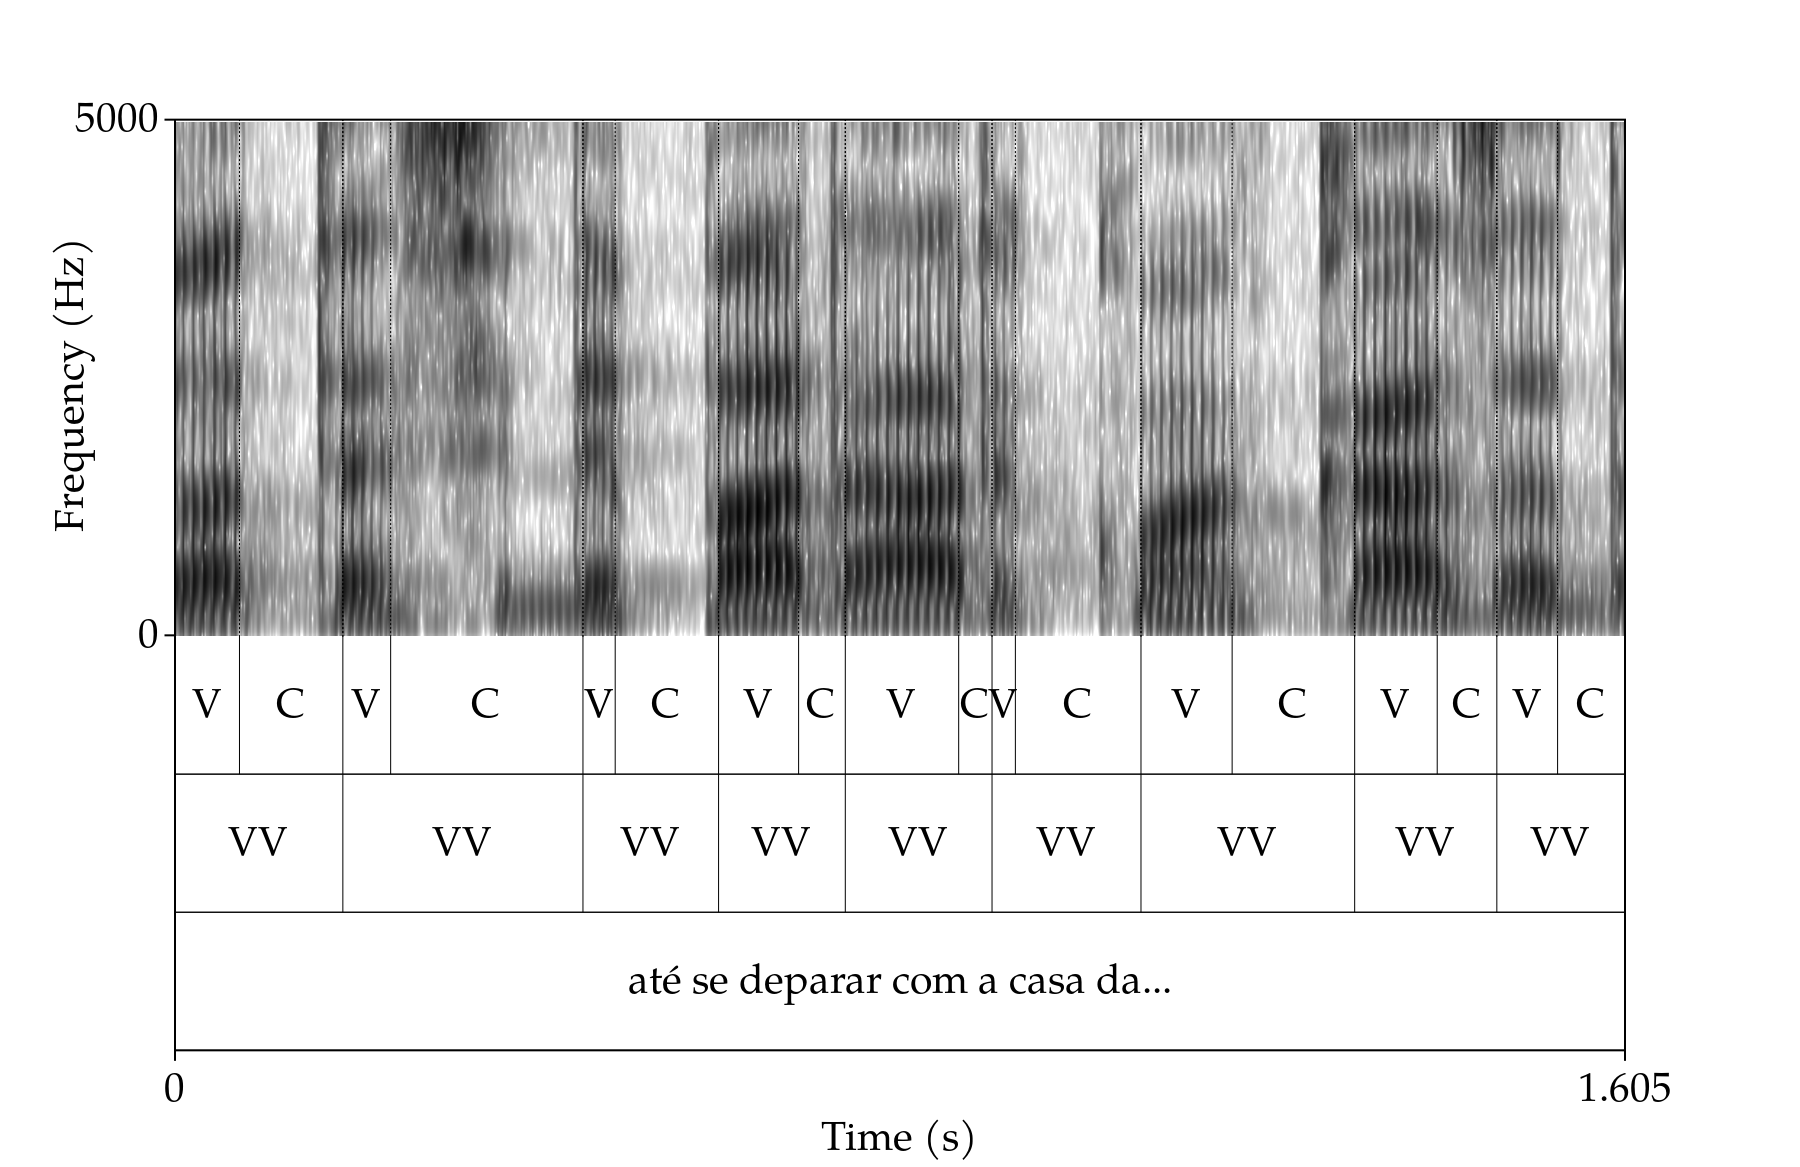
\includegraphics{praat_sample_01}
	\end{figure} %%%ref da imagem? 
		
	\subsection{Medições acústicas} \label{medicoes}

	Quando as amostras já estiverem devidamente segmentadas e etiquetadas, as
	métricas rítmicas já poderão ser calculadas. Isso será feito de modo
	completamente automático por meio do algoritmo \emph{Metrics and Acoustics
		Extractor} desenvolvido recentemente por \citet{Junior.Barbosa2019} para
	ser executado no Praat. Basicamente, esse algoritmo aplica as equações
	matemáticas de cada métrica às durações dos intervalos segmentados
	previamente e então gera uma planilha organizada com os índices rítmicos de
	cada enunciado selecionado\footnote{Portanto, o número de valores gerados
		por cada métrica de ritmo será o número total de enunciados. No caso
		desta pesquisa, cada métrica irá gerar em torno de 1.260 valores.}.

	As principais métricas de ritmo que foram elaboradas até então consistem,
	basicamente, em dois tipos de cálculos aplicados a durações de certos
	intervalos: (i) cálculo de proporção; (ii) e cálculo de dispersão. As
	métricas do primeiro grupo são operações simples que determinam a
	porcentagem do enunciado que é composta por um certo tipo de intervalo. Por
	exemplo, a métrica $\%V$ \citep{Ramus.etal1999} calcula a porcentagem do
	enunciado que é composta por intervalos vocálicos. Já as métricas do segundo
	grupo consistem em algum tipo de medida de dispersão, como o desvio padrão,
	que calcula a variabilidade na duração de algum tipo de intervalo do
	enunciado. Por exemplo, a métrica $\Delta C$ \citep{Ramus.etal1999} nada
	mais é do que a aplicação do desvio padrão às durações dos intervalos
	consonantais de um enunciado. Valores mais altos dessa métrica indicam que
	esses intervalos são mais variáveis e vice-versa. As principais diferenças
	entre as métricas são o tipo de intervalo a que se aplicam, qual cálculo de
	dispersão adotam (no caso do segundo grupo) e se utilizam alguma forma de
	normalização da taxa de elocução. %Um resumo das métricas que serão
	%usadas nesta pesquisa pode ser visualizado no Apêndice \ref{metricas} .%%%Não é muito bom ter anexo em projeto, a menos que imprescindível!

	\section{Formas de análise dos resultados} \label{analise}

	Como resultado da extração automatizada das medidas rítmicas, se obterá uma
	planilha já organizada com os valores de todas as métricas para cada um dos
	enunciados que compõem as amostras, sendo que o informante que produziu cada
	enunciado já estará devidamente identificado na planilha junto com as
	informações acerca da sua idade de migração e seu tempo de residência em São
	Paulo. A partir dessa planilha e com o uso da plataforma R
	\citep{RCoreTeam2019}, serão realizadas análises e testes estatísticos (em
	especial, modelos de regressão linear de efeitos mistos) para investigar a
	distribuição dos valores rítmicos obtidos em função das variáveis Idade de
	Migração e Tempo de Residência. Além disso, também serão realizadas análises
	estatísticas para determinar as diferenças nos valores rítmicos entre a
	amostra de interesse e as de controle. 
	
	{\setstretch{1.3} % Espaçamento entre linhas
		\printbibliography
	}

\begin{comment}
%%%Guarde a tabela abaixo para relatórios e a própria dissertação. Aqui, num projeto, ela parece "fora de lugar". Como conversamos, não é seu papel "ensinar" ao parecerista sobre prosódia (vc pode acabar fazendo isso no desenvolver da pesquisa, na dissertação). Aqui, seu papel é convencer o leitor de que a pesquisa vale a pena ser feita. Tudo o que for necessário para entender seus objetivos e métodos tem que estar explicado no texto. 

\pagebreak

\appendix
\section{Métricas de ritmo}

\begin{table}[h] 
	\label{metricas}	
	\caption{\normalsize Métricas de ritmo} 
	\vspace{1em}

		
\begin{tabular}{m{54mm} m{62mm} m{41.4mm}}
		
\scshape\normalsize Parâmetro & \scshape\normalsize Descrição &
\scshape\normalsize Principal referência \\

\hline
\hline

Percentual (\%) & Porcentagem total do enunciado composto pelos intervalos vocálicos (\%V) ou consonantais (\%V) & \cite{Ramus.etal1999} \\

\rowcolor{cinza1} Desvio padrão ($\Delta$) &  Desvio padrão dos intervalos vocálicos ($\Delta$V), consonantais ($\Delta$C), vocálico-consonantais ($\Delta$S) ou silábicos ($\Delta$S) & \cite{Ramus.etal1999}  \\

Coeficiente de variabilidade (Varco) &  Desvio padrão dos intervalos\textsuperscript{a} dividido pela média e multiplicado por 100 & \cite{Dellwo2006}\\

\rowcolor{cinza1} Índice de variabilidade em pares não normalizado (rPVI) & Média aritmética das diferenças de duração entre intervalos adjacentes & \cite{Low.etal2000} \\

Índice de variabilidade em pares normalizado (nPVI) & Média arimética das diferenças de duração entre intervalos adjacentes com normalização tipo 1 & \cite{Low.etal2000} \\

\rowcolor{cinza1} Quociente rítmico (RR)  & Média aritmética dos quocientes de duração entre intervalos adjacentes & \cite{Gibbon.Gut2001}  \\

Índice de variabilidade (VI)  &  Média aritmética das diferenças de duração entre intervalos adjacentes com normalização tipo 2 & \cite{Deterding1994, Deterding2001} \\

\rowcolor{cinza1} PVI normalizado com \emph{z-score} (YARD) & Média aritmética dos quocientes de duração entre intervalos adjacentes com normalização em \emph{z-score} & \cite{Wagner.Dellwo2015} \\

\hline \hline 

	\multicolumn{3}{m{.97\linewidth}}{\textsuperscript{a}Todas essas
	métricas têm versões correspondentes à sua aplicação aos seguintes
	intervalos: intervalos vocálicos (V), intervalos consonantais (C),
	intervalos vocálico-consonantais (VC) e intervalos silábicos (S). O
	intervalo vocálico-consonantal equivale ao que se chama de intervalo entre
	início de vogais ou intervalo VV.} \\ 
\end{tabular}  
\end{table}
\end{comment}

	\end{document}
